\documentclass{article}
\usepackage[utf8]{inputenc}

\title{Report.4.threads.tex}
\author{gw.muraro}
\date{November 1st 2018}

\usepackage{natbib}
\usepackage{graphicx}
\usepackage{pgfplots}
\usepackage{minted}

\begin{document}

\maketitle
\section{Labwork 4}
\subsection{Explain how you improve the labwork}

    As we work on basicly a precedent code, we will copy paste a huge amount of code from the labwork 3 function. But we will do some modification. 
    
    
    \begin{enumerate}

    \item Modifications on block size and grid size
    \begin{minted}{c}
        // block number is a parameter equals to 32 by default
         dim3 gridSize = dim3(inputImage->width / blockNumber, inputImage->height / blockNumber);
        dim3 blockSize2 = dim3(blockNumber, blockNumber);
    \end{minted}

    \item Modification of the Kernel call with good arguments 
    \begin{minted}{c}
        grayScale<<<gridSize, blockSize2>>>(devInput, devGray) ;    
    \end{minted}

    \item Modification of the kernel to a 2D process
    \begin{minted}{c}
        
        int tid = (threadIdx.x + blockIdx.x * blockDim.x) + 
                  totalWidth * (threadIdx.y + blockIdx.y * blockDim.y);
        output[tid].x = (input[tid].x + input[tid].y + input[tid].z) / 3;
        output[tid].z = output[tid].y = output[tid].x;

    \end{minted}

    \end{enumerate}    
\subsection{What is the speedup}
\begin{verbatim}
    ==== labwork 1 ../data/eiffel.jpg
    USTH ICT Master 2018, Advanced Programming for HPC.
    Warming up...
    Starting labwork 1
    labwork 1 CPU ellapsed 3001.4ms
    ==== labwork 4 ../data/eiffel.jpg 1
    USTH ICT Master 2018, Advanced Programming for HPC.
    Warming up...
    Starting labwork 4
    labwork 4 ellapsed 116.4ms
    ==== labwork 4 ../data/eiffel.jpg 2
    USTH ICT Master 2018, Advanced Programming for HPC.
    Warming up...
    Starting labwork 4
    labwork 4 ellapsed 105.9ms
    ==== labwork 4 ../data/eiffel.jpg 4
    USTH ICT Master 2018, Advanced Programming for HPC.
    Warming up...
    Starting labwork 4
    labwork 4 ellapsed 103.5ms
    ==== labwork 4 ../data/eiffel.jpg 16
    USTH ICT Master 2018, Advanced Programming for HPC.
    Warming up...
    Starting labwork 4
    labwork 4 ellapsed 103.0ms
    ==== labwork 4 ../data/eiffel.jpg 32
    USTH ICT Master 2018, Advanced Programming for HPC.
    Warming up...
    Starting labwork 4
    labwork 4 ellapsed 102.5ms

\end{verbatim}
\subsection{Plot a graph of block size vs speedup}
    
    %%plot
    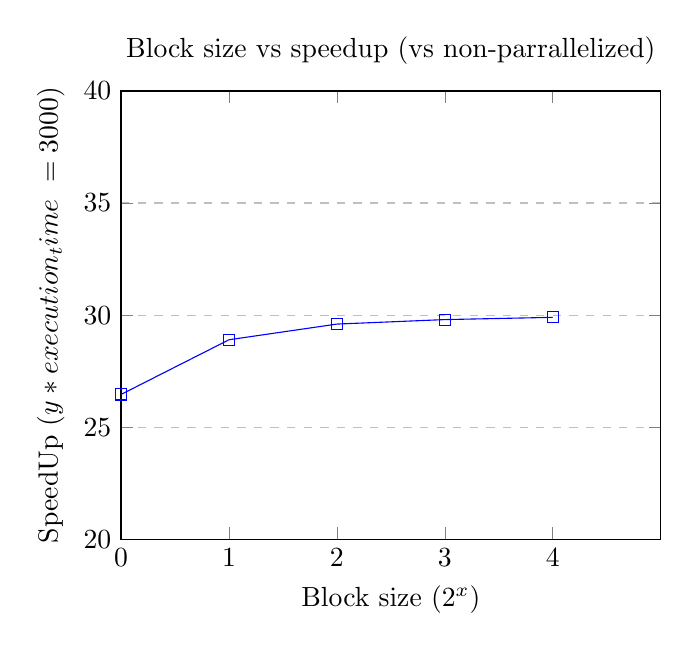
\begin{tikzpicture}
        \centering
        %%define axes
        \begin{axis}[
            title={Block size vs speedup (vs non-parrallelized)},
            xlabel={Block size ($2^x$)},
            ylabel={SpeedUp ($y*execution_time ~= 3000$)},
            xmin=0, xmax=5,
            ymin=20, ymax=40,
            xtick={0,1,2,3,4},
            ytick={20, 25, 30, 35, 40},
            legend pos=north west,
            ymajorgrids=true,
            grid style=dashed,
        ]
        %% data filing
        \addplot[
            color=blue,
            mark=square,
            ]
            coordinates { %% Remind : axis X = 2^x
                (0,26.46)(1,28.9)(2,29.6)(3,29.8)(4,29.9)
            };
        

        \end{axis}
    \end{tikzpicture}
    \newline
    


\end{document}

